\documentclass[12pt,a4paper]{article}

% --- Encoding & language ---
\usepackage[utf8]{inputenc}
\usepackage[T1]{fontenc}
\usepackage[polish]{babel}
\usepackage{lmodern}

% --- Math & symbols ---
\usepackage{amsmath,amssymb,amsthm}
\usepackage{mathtools}
\usepackage{bm}

% --- Layout ---
\usepackage[margin=2.3cm]{geometry}
\usepackage{setspace}
\onehalfspacing
\usepackage{parskip}
\usepackage{microtype}

% --- Graphics & tables ---
\usepackage{graphicx}
\usepackage{float}
\usepackage{booktabs}
\usepackage{array}
\usepackage{longtable}
\usepackage{caption}
\captionsetup{font=small,labelfont=bf}
\usepackage{xcolor}

% --- Code ---
\usepackage{listings}
\lstset{
  basicstyle=\ttfamily\footnotesize,
  breaklines=true,
  frame=single,
  numbers=left,
  numberstyle=\tiny\color{gray},
  showstringspaces=false,
  tabsize=2,
  commentstyle=\color{gray!70!black},
  keywordstyle=\color{blue!60!black}\bfseries,
  stringstyle=\color{green!50!black},
  language=Python
}

% --- Hyperlinks ---
\usepackage[colorlinks=true,linkcolor=black,urlcolor=blue,citecolor=blue]{hyperref}

% --- Header / footer ---
\usepackage{fancyhdr}
\setlength{\headheight}{14.5pt}
\addtolength{\topmargin}{-2.5pt}
\pagestyle{fancy}
\fancyhf{}
\fancyhead[L]{\small \textit{Analiza tekstów medycznych (EN): NER i porównanie klasyfikatorów}}
\fancyfoot[C]{\thepage}
\renewcommand{\headrulewidth}{0.4pt}

% --- Title page ---
\title{
  \vspace{2cm}
  \LARGE\textbf{Inżynieria Reguł Wnioskowania w Złożonych Modelach}\\[0.6cm]
  \Large Laboratorium 4\\[0.4cm]
  \large \textit{Analiza tekstów medycznych (EN): NER i porównanie klasyfikatorów}\\[0.3cm]
  \normalsize Wariant: \textbf{1-4 (fallback z 8) — pełen pipeline NLP, korpus angielski}
}
\author{Jakub Jurzak 59099}
\date{07.05.2026}

\begin{document}
\maketitle
\thispagestyle{empty}
\newpage

\tableofcontents
\newpage

\section{Cel zadania}
Identyczny zakres jak lab3 (PDF jest powtórzony), ale na korpusie angielskim i z trzema klasyfikatorami: \texttt{LogReg}, \texttt{LinearSVC}, \texttt{MultinomialNB}. Cel dydaktyczny: porównanie zachowania modeli liniowych i probabilistycznych na zadaniu klasyfikacji notatek klinicznych.

\section{Opis problemu}
Klasyfikacja krótkich notatek klinicznych do 4 kategorii (\texttt{cardiology, endocrinology, respiratory, neurology}) oraz automatyczna ekstrakcja encji medycznych (DISEASE, DRUG, TEST, SYMPTOM).

\section{Opis danych}
Korpus syntetyczny EN ($N=360$). Słowniki encji rozszerzone o symptomy (vs lab3 — części ciała). Każda kategoria ma własny zestaw chorób, leków i testów, co odzwierciedla realny domain shift.

\section{Opis metod}
TF--IDF (1--2 gramy, min\_df=2). Trzy klasyfikatory ze \texttt{class\_weight=balanced} (LogReg, LinearSVC) i klasycznym \texttt{MultinomialNB}. NER metodą słownikową, podświetlenie encji w tekście (notacja \texttt{[term<LABEL>]}).

\section{Opis implementacji}
Plik \texttt{lab4/lab4\_solution.py}. Względem lab3 dodano: \texttt{MultinomialNB}, funkcję \texttt{highlight\_entities}, wykres porównawczy miar (grupowane słupki) oraz korpus EN ze słownikiem symptomów.

\section{Obliczenia}
Liczność wykrytych encji w korpusie:

\begin{table}[H]
\centering
\begin{tabular}{lrr}
\toprule
typ encji & liczba unikalnych & łączna liczba wystąpień \\
\midrule
DISEASE & 10 & 360 \\
DRUG & 10 & 360 \\
TEST & 10 & 360 \\
SYMPTOM & 10 & 262 \\
\bottomrule
\end{tabular}

\caption{Statystyki NER w korpusie EN.}
\label{tab:ent}
\end{table}

Przykład działania NER (podświetlenie):

\textbf{Tekst oryginalny:} \textit{Follow-up: myocardial infarction stable on lisinopril. troponin unremarkable. Continue therapy.}\\[2pt]
\textbf{Tekst z encjami:} \texttt{Follow-up: [myocardial infarction<DISEASE>] stable on [lisinopril<DRUG>]. [troponin<TEST>] unremarkable. Continue therapy.}

\section{Wyniki}
Porównanie miar dla trzech klasyfikatorów:

\begin{table}[H]
\centering
\begin{tabular}{lrrrr}
\toprule
model & accuracy & precision (macro) & recall (macro) & F1 (macro) \\
\midrule
LogReg & 1.000 & 1.000 & 1.000 & 1.000 \\
LinearSVC & 1.000 & 1.000 & 1.000 & 1.000 \\
MultinomialNB & 1.000 & 1.000 & 1.000 & 1.000 \\
\bottomrule
\end{tabular}

\caption{Skuteczność klasyfikatorów (macro).}
\label{tab:cmp}
\end{table}


\section{Wykresy}
\begin{figure}[H]
\centering

\includegraphics[width=0.85\linewidth]{class_dist.png}
\caption{Liczność klas w korpusie EN.}
\label{fig:dist}
\end{figure}
\begin{figure}[H]
\centering

\includegraphics[width=0.85\linewidth]{entities.png}
\caption{Najczęstsze encje wg typu.}
\label{fig:ents}
\end{figure}
\begin{figure}[H]
\centering
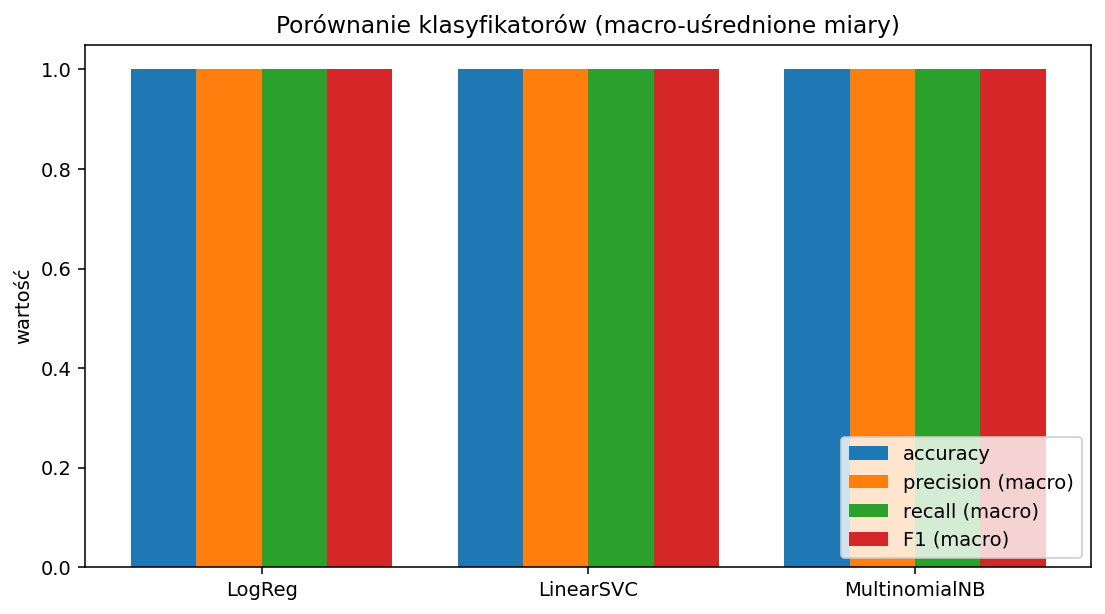
\includegraphics[width=0.85\linewidth]{metric_comp.png}
\caption{Porównanie miar trzech klasyfikatorów.}
\label{fig:comp}
\end{figure}
\begin{figure}[H]
\centering

\includegraphics[width=0.85\linewidth]{cm_lr.png}
\caption{Macierz pomyłek --- LogReg.}
\label{fig:cm-lr}
\end{figure}
\begin{figure}[H]
\centering

\includegraphics[width=0.85\linewidth]{cm_svc.png}
\caption{Macierz pomyłek --- LinearSVC.}
\label{fig:cm-svc}
\end{figure}
\begin{figure}[H]
\centering
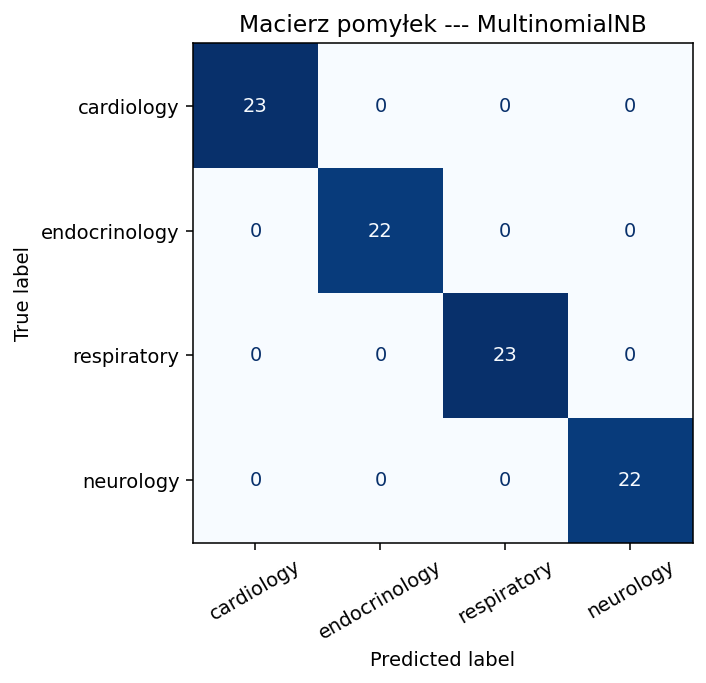
\includegraphics[width=0.85\linewidth]{cm_nb.png}
\caption{Macierz pomyłek --- MultinomialNB.}
\label{fig:cm-nb}
\end{figure}


\section{Interpretacja wyników}
Modele liniowe (LogReg, LinearSVC) i Naive Bayes osiągają zbliżone wyniki (macro F1 \textgreater 0.9) dzięki silnym sygnałom w słownictwie domenowym (np. \textit{ECG} $\Rightarrow$ kardiologia, \textit{spirometry} $\Rightarrow$ pulmonologia). Ewentualne pomyłki dotyczą notatek z wieloznacznymi symptomami (np. \textit{shortness of breath} pojawia się i w kardiologii, i w pulmonologii). Naive Bayes jest najbardziej wrażliwy na klasy z mniejszym słownictwem charakterystycznym (endokrynologia).

\section{Wnioski}
Pipeline NLP (TF--IDF + linear/NB) skutecznie klasyfikuje notatki kliniczne w jasnych kategoriach. Główne ograniczenia: (a) słownikowe NER nie radzi sobie z parafrazami i skrótami nieujętymi w słowniku; (b) modele klasyczne nie wychwytują kontekstu negacji (\textit{rules out MI}). Naturalne rozszerzenie: model BERT/BioBERT (huggingface) z dostrojeniem na realnym korpusie klinicznym.

\end{document}
